\documentclass[xcolor={dvipsnames}]{beamer}

\mode<presentation> {
    \usepackage[utf8]{inputenc}
    \usepackage[T1]{fontenc}
    \usepackage[brazil]{babel}
    \usepackage{csquotes}
    \usepackage{float}
    \usepackage{verbatim}

    \bibliographystyle{plain}

    \usetheme{Madrid}
    \usecolortheme{ipbutfpr}

    \setbeamertemplate{caption}[numbered]
    \setbeamertemplate{bibliography item}{\insertbiblabel}
    \setbeamertemplate{frametitle continuation}{\gdef\beamer@frametitle{}}

    \setbeamertemplate{footline}{
        \leavevmode%
        \hbox{%
            \begin{beamercolorbox}[wd=.4\paperwidth,ht=2.25ex,dp=1ex,center]{author in head/foot}%
                \usebeamerfont{author in head/foot}\insertshortauthor
            \end{beamercolorbox}%
            \begin{beamercolorbox}[wd=.6\paperwidth,ht=2.25ex,dp=1ex,center]{title in head/foot}%
                \usebeamerfont{title in head/foot}\insertshorttitle\hspace*{6em}
                \insertframenumber{} / \inserttotalframenumber\hspace*{1ex}
            \end{beamercolorbox}
        }%
        \vskip0pt%
    }

    \setbeamertemplate{navigation symbols}{}
}

\usepackage[language=brazil, style=numeric, sorting=none]{biblatex}
\addbibresource{main.bib}
\makeatletter

\makeatother

\title[Proyectos I]{ Metodologías de Investigación en Ciencias de la Computación}

\author[Humpire Hayde - Salcedo Melvin]{ Humpire Cutipa Hayde Luzmila, Salcedo Almiron Melvin David}

\institute[IPB]{\normalsize
    Dr.(c) Wilber Ramos Lovon  

    \begin{figure}[H]
        \centering
        
\includegraphics[width=0.17\textwidth]{images/Unsa.png}
        %
\includegraphics[width=0.4\textwidth]{images/cs.png}
    \end{figure}
}
\date{\small Escuela Profesional de Ciencia de la Computación \\ 20 de Mayo de 2019}

%Arquitectura
%Metodo de procesamiento
%Metodo de almacenamiento
%Resultados
%Conclusiones
%Consumo de recursos, arquitectura de la lap? 


\begin{document}
    \frame{\titlepage}
    
    %----SLIDES----%
    \begin{frame}{Tabla de Contenidos}
        \tableofcontents
    \end{frame}
    
    \section{Introducción}
    \begin{frame}{Ciencia de la computación}


\begin{block}{Ciencia}
\begin{itemize}
    \item La ciencia es un cuerpo de conocimiento organizado o sistemático. La ciencia abarca muchos dominios diferentes, sin embargo, esos dominios están relacionados. [1].
\end{itemize}
\end{block} 
        
\begin{block}{Ciencia de la computación}
\begin{itemize}
     \item Con respecto a la informática (CS), algunos dijeron que no debería llamarse ciencia.
    \item CS es transversal a dominios muy diferentes y es un gran tema de investigación científica.
\end{itemize}
\end{block}   
        

\end{frame}

\begin{frame}{Ciencia de la computación}
\begin{figure}[H]
    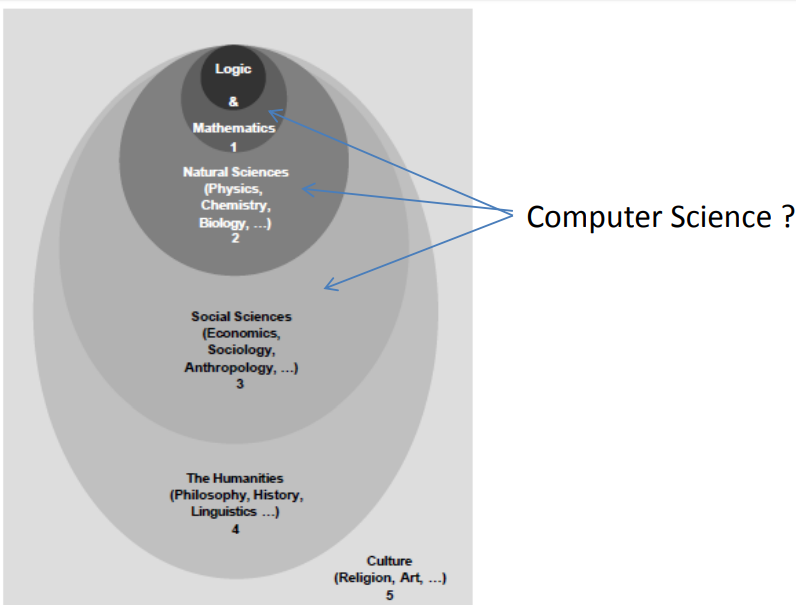
\includegraphics[scale=0.4]{images/figura1.PNG}
    \caption{Ciencia de la computación [1]}
    \label{fig:boat1}
\end{figure} 
\end{frame}

\begin{frame}{La Investigación}
\begin{block}{La investigación}
La investigación es un estudio cuidadoso, sistemático, paciente y una investigación en algún campo del conocimiento, realizado para establecer hechos. [1]
\end{block} 
\end{frame}


\begin{frame}{La Metodología}
\begin{block}{La metodología}
La metodología es la estrategia general que describe la forma en que se debe emprender el proyecto y, entre otras cosas, identifica los métodos que se utilizarán en él. [1]
\end{block} 
\begin{exampleblock}{}
\begin{itemize}
    \item Los investigadores de ciencias de la computación utilizan varias metodologías para abordar preguntas dentro de la disciplina. 
    \item Las tareas realizadas por un solo investigador se encuentran dentro de diferentes metodologías. Incluso las actividades requeridas para abordar una única pregunta de investigación pueden incluir varias de estas metodologías.
\end{itemize}
\end{exampleblock}
\end{frame}

\begin{frame}{Metodologías de búsqueda}
\begin{block}{Metodologías de la investigación. [2]}
\begin{itemize}
\item \textbf{En un contexto académico}: La investigación se utiliza para referirse a la actividad de una investigación o investigación diligente y sistemática en un área, con el objetivo de descubrir o revisar hechos, teorías, aplicaciones. 
\item [--] \textbf{El objetivo} es descubrir y difundir nuevos conocimientos. (existen varios métodos que se pueden usar en CS en la siguiente diapositiva que mostraremos estas metodologías).
\end{itemize}
\end{block} 
\end{frame}

\begin{frame}{Métodos que se pueden usar en Ciencia de la Computación}
\begin{figure}[H]
    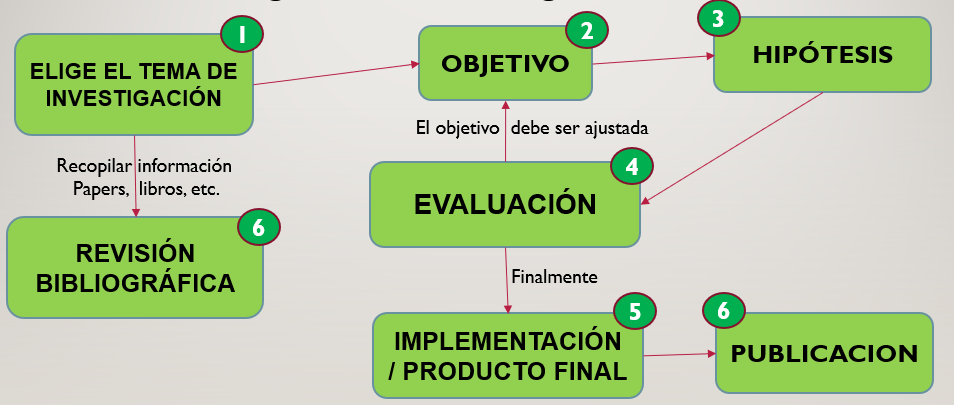
\includegraphics[scale=0.48]{images/figura3.PNG}
    \label{fig:boat1}
\end{figure}     
\end{frame}

\begin{frame}{Diagrama2 : Metodologías científicas en Cs}
 \begin{figure}[H]
    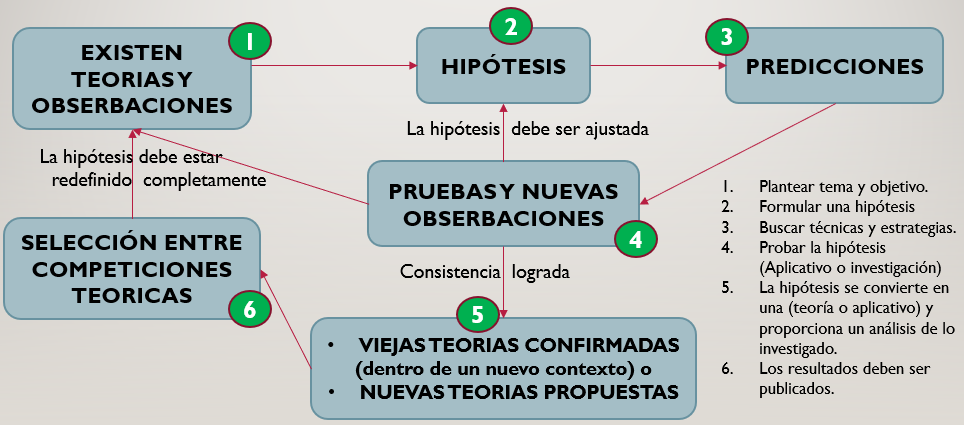
\includegraphics[scale=0.48]{images/figura5.PNG}
    \label{fig:boat1}
\end{figure}    
\end{frame}
    
    \section{Tipos de metodologías de investigación en Cs}
    \subsection{Metodologías formales}
    \subsection{Metodologías experimentales}
    \subsection{Metodologías de construcción}
    \subsection{Metodologías de procesos}
    \subsection{Metodologías de modelo}
    \begin{frame}{Tipos de metodologías de investigación en Cs}
 \begin{figure}[H]
    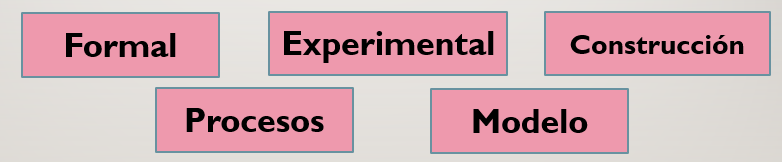
\includegraphics[scale=0.58]{images/figura2.PNG}
    \label{fig:boat1}
\end{figure}     
\end{frame}

\begin{frame}{Metodologías formales}
\begin{block}{}
\begin{itemize}
    \item Prueba hechos sobre algoritmos y sistemas. 
    \item Estas metodologías están más orientadas hacia la ciencia de la computación teórica. [1]
    \item Generalmente se ocupa del modelado y la abstracción. 

    \item Preguntas en  ciencias de la computación:
    \begin{itemize}
        \item Dado un problema X.
            \begin{itemize}
        \item ¿Qué tan difícil es resolverlo? (computabilidad)
        \item ¿Cuánto tiempo/espacio tarda? (complejidad)
        \item¿Cuáles son sus limitaciones? 
        \item Dado un formalismo, ¿qué puede expresar?
    \end{itemize}
    \end{itemize}
\end{itemize}
 \end{block} 
\end{frame}


\begin{frame}{Metodologías experimentales}
\begin{block}{}
\begin{itemize}
    \item Evaluar nuevas soluciones para problemas.[1]
    \item División:
    \begin{itemize}
        \item Fase exploratoria: Son las preguntas que se deben hacer sobre el sistema que se está evaluando. 
        \item Fase de evaluación: intentará responder estas preguntas. Un experimento bien diseñado comenzará con una lista de las preguntas que se espera que el experimento responda.
    \end{itemize}
\end{itemize}
 \end{block} 
\end{frame}

\begin{frame}{Metodologías de construcción}
\begin{block}{}
\begin{itemize}
    \item Consiste en construir un artefacto [1].
    \begin{itemize}
        \item Ya sea un artefacto físico o un sistema de software, para demostrar que es posible. 
    \end{itemize}
    \item Para ser considerada investigación, la construcción del artefacto debe ser nueva o debe incluir nuevas características que no se hayan demostrado anteriormente en otros artefactos.
\end{itemize}
 \end{block} 
\end{frame}

\begin{frame}{Metodologías de procesos}
\begin{block}{}
  \begin{itemize}
    \item Comprender los procesos utilizados para realizar tareas en  Ciencias de la computación. [1]
    \item Esta metodología se utiliza principalmente en las áreas de Ingeniería de software y Interfaz hombre-máquina, que se ocupan de la forma en que los humanos construyen y utilizan los sistemas informáticos. 
\end{itemize}  
 \end{block} 
\end{frame}

\begin{frame}{Metodologías de modelo}
\begin{block}{}
Los experimentos basados en un modelo se llaman simulaciones. Cuando se crea una descripción formal del modelo para verificar la funcionalidad o la corrección de un sistema, la tarea se denomina verificación de modelo.[1]
\begin{itemize}
    \item Centra en definir un modelo abstracto para un sistema real. Este modelo será mucho menos complejo que el sistema que modela y, por lo tanto.
    \item Permitirá al investigador comprender mejor el sistema y utilizar el modelo para realizar experimentos que no podrían realizarse en el propio sistema debido al costo o la accesibilidad. 
    \item Se utiliza a menudo en combinación con las otras cuatro metodologías.
\end{itemize} 
 \end{block} 
\end{frame}

    
    
    \section{Punto de partida de la investigación}
    \subsection{Elegir tema}
    \subsection{Planteamiento del problema}
    \subsection{Hipótesis y variables de la investigación}
    \subsection{Objetivos de la investigación}
    \subsection{Evaluación y implementación}
    \begin{frame}{Punto de partida de la investigación}
\begin{block}{}
Consiste en hallar, formular problemas y luchar con ellos:
\begin{itemize}
    \item Criticar soluciones o problemas conocidos o existentes.
    \item Aplicar soluciones innovadoras a problemas conocidos o existentes o proponer soluciones conocidas a problemas innovadores.
    \item Buscar nuevas relaciones entre problemas ya conocidos.
    \item Abordar problemas ya conocidos desde distintos campos.
\end{itemize}
\end{block} 
\end{frame}
        
\begin{frame}{Elegir el tema de investigación}
\begin{block}{}
\begin{itemize}
    \item La elección se puede hacer buscando:
    \begin{itemize}
        \item Relevante:  Científico, social, tecnológico.
        \item Adecuado:  Para los empleados en la universidad, instituto y laboratorio de investigación.
    \end{itemize}
    \item Consultar tiempo y viabilidad para desarrollar la investigación. 
    \begin{itemize}
        \item Ámbito: No es necesario resolverlo todo. Es mejor limitarse luego ser demasiado amplio.
    \end{itemize}
\end{itemize}
\end{block} 
\end{frame}

\begin{frame}{Revisión bibliográfica}
\begin{block}{}
\begin{itemize}
    \item Está bien comenzar con libros y papers. Después de dominar las técnicas principales, busque trabajo relevante en buenos repositorios
    \item Puedes buscar exclusivamente en (Top Computer Science Conferences).
    \item Repositorios de busqueda:
    \begin{itemize}
        \item Scholar (http://scholar.google.com) 
        \item Scopus (http://www.scopus.com)
        \item  Web of Science (http://www.webofknowledge.com)
    \end{itemize}
\end{itemize}
\end{block}
\end{frame}

\begin{frame}{Planteamiento del problema}
\begin{block}{}
Es la explicación de tu tema o de lo que quieres hacer en tu trabajo, pero no funciona de esa manera. Se trata de establecer la problemática de tu investigación. 
\begin{itemize}
    \item ¿Eso qué quiere decir? Debes concretar una situación para analizarla, delimitarla, describirla y darle una posible solución o respuesta al por qué de sus causas o consecuencias.
\end{itemize}
\end{block}   
\end{frame}

\begin{frame}{Pregunta de investigación}
\begin{block}{}
 La pregunta principal de investigación es la pregunta que tu tesis pretende responder y deriva del planteamiento del problema que has formulado previamente. 
\end{block}   
\end{frame}

\begin{frame}{Hipótesis}
\begin{block}{}
\begin{itemize}
    \item  Es una posible solución al problema. quienes afirman que es un método de comprobación. [1]
    \item [--] Los buenos objetivos son impulsados por una buena hipótesis de investigación.
    \item [--] Definir una hipótesis sólida es lo que diferencia la investigación de un trabajo técnico.
\end{itemize}
\end{block} 
\end{frame}

\begin{frame}{Variables de la investigación}
\begin{block}{}
La clave para diseñar cualquier experimento o aplicaciones es ver qué variables de investigación podrían afectar el resultado. [1]
 \begin{itemize}
     \item Variable Independiente: Es el centro del experimento y desarrollada por el investigador.
     \item Variable Dependiente: Es el resultado medible de este desarrollo, los resultados experimentales o aplicaciones.
 \end{itemize}
\end{block}  
\end{frame}

\begin{frame}{Objetivos de la investigación}
\begin{block}{}
\begin{itemize}
    \item El objetivo se puede definir con una revisión tecnológica. [1]
    \item Debe ser una acción que solucione algún problema o problema existente.
    \item Debe ir acompañado de una hipótesis bien definida
\end{itemize}
\end{block}
 \begin{figure}[H]
    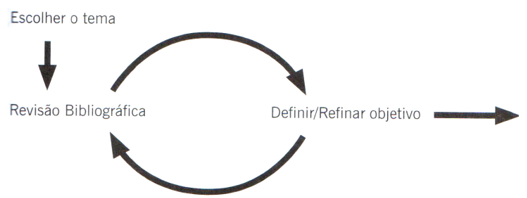
\includegraphics[scale=0.55]{images/figura4.PNG}
    \label{fig:boat1}
\end{figure}
\end{frame}

\begin{frame}{Evaluación}
\begin{block}{}
 \begin{itemize}
     \item ¿Cómo evaluar tu investigación?	
    \begin{itemize}
        \item Defina, lo antes posible, cómo medir sus resultados para entender qué tan cerca está del objetivo principal.
        \begin{itemize}
            \item Me esfuerzo mucho, pero si es necesario, suelta / cambia la idea inicial.
        \end{itemize}
    \end{itemize}
    \item Dado que generalmente el 90\% de los resultados son realmente fallos, debemos asegurarnos de que estamos evaluando correctamente los resultados, desde el principio
    \begin{itemize}
        \item Comprender que toda investigación tiene limitaciones y puntos débiles.
    \end{itemize}
 \end{itemize}  
 \end{block}
\end{frame}

\begin{frame}{Implementación}
\begin{block}{}
\begin{itemize}
    \item Puedo ser innovador o no.
    \item Si falta una hipótesis, entonces no es así.
    \item Cuando es innovador, suele ser explorador.
    \item Si se trata de un sistema o reproducción, puede informarse en un “Informe técnico”.
    \item Aceptable para proyectos finales de pregrado (TCC), pero difícilmente para maestrías o doctorados
\end{itemize}
\end{block}
\end{frame}



    \section{Publicación de un articulo}
    \subsection{Estructura del articulo}
    \subsection{Donde publicar}
    \begin{frame}{Publicación de un articulo}
\begin{block}{Articulo}
Es comunicar los resultados de investigaciones, ideas, debates, mejoras de manera clara, concisa y fiable.
\end{block}  
\begin{figure}[H]
    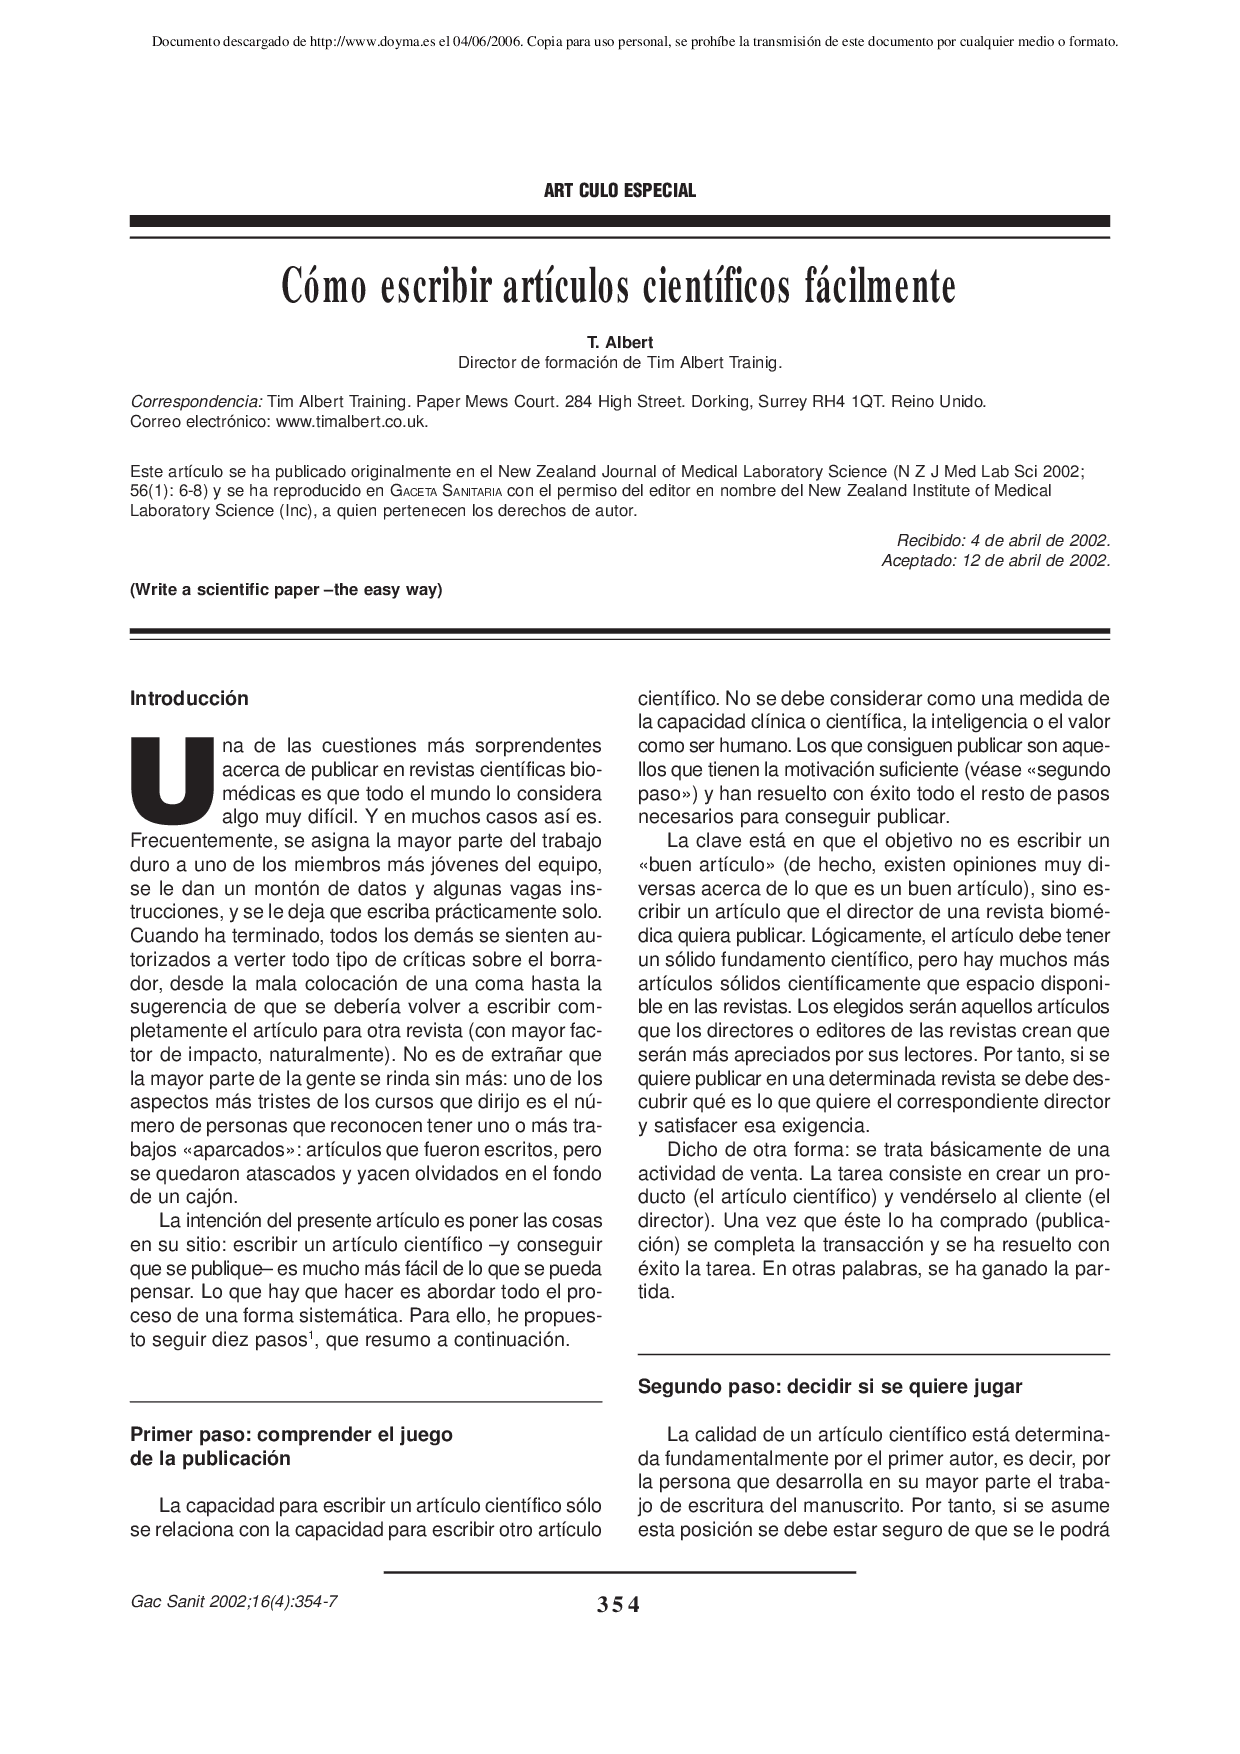
\includegraphics[scale=0.09]{images/articulo.png}
    \label{fig:boat1}
\end{figure}
\end{frame}


\begin{frame}{Revista Indexada}
\begin{block}{}
Publicación periódica de investigación demuestra que una alta calidad ha sido listada en alguna base de datos mundial.
\end{block}   
\begin{figure}[H]
    
\includegraphics[scale=0.4]{images/revistaindexada.png}
    \label{fig:boat1}
\end{figure}
\end{frame}

\begin{frame}{Proceso}
\begin{block}{}
\begin{enumerate}
    \item Desarrollar un plan (temas de interés)
    \item Elegir una revista
    \item Escribir un articulo
    \item Enviar
    \item Revisar
\end{enumerate}
\end{block}   
\end{frame}

\begin{frame}{Desarrollo del plan}
\begin{block}{Tema de interés}
\begin{itemize}
    \item Elementos originales de tu tesis?
    \item Contribución a la ciencia
    \item Pregunta de investigación
\end{itemize}
\end{block}   
\end{frame}

\begin{frame}{Búsqueda en la Web de Sciense}
\begin{block}{Web de Sciense}
El objetivo es seguir impulsando el uso de la herramienta y dar a conocer las últimas novedades introducidas. [4]
\end{block}   
\begin{figure}[H]
    
\includegraphics[scale=0.4]{images/webcite.png}
    \label{fig:boat1}
\end{figure}
\end{frame}

\begin{frame}{Búsqueda en scimagojr.com}
\begin{block}{scimagojr.com}
Scimago Institutions Ranking clasifica instituciones directamente vinculadas a la investigación y las posiciona a través de un indicador de síntesis combinando una serie de variables que pertenecen a tres grandes ámbitos: Investigación, Innovación, Impacto social, medido, este último, a través de la visibilidad de sus webs. [6]
\end{block}   
\begin{figure}[H]
    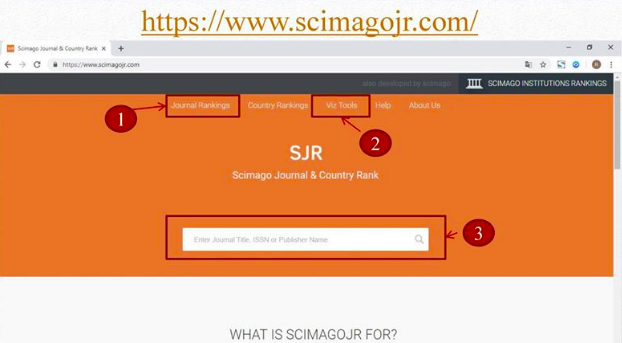
\includegraphics[scale=0.4]{images/webcite2.png}
    \label{fig:boat1}
\end{figure}
\end{frame}

\begin{frame}{Búsqueda en Top Computer Science Conferences}
\begin{block}{Top Computer Science Conferences}
Información de la conferencia, clasificación de la conferencia y métricas (esta es una conferencia TOP). Para hacer la busqueda podemos filtrar por áreas de nuestro interés y por países. [5]
\end{block}   
\begin{figure}[H]
    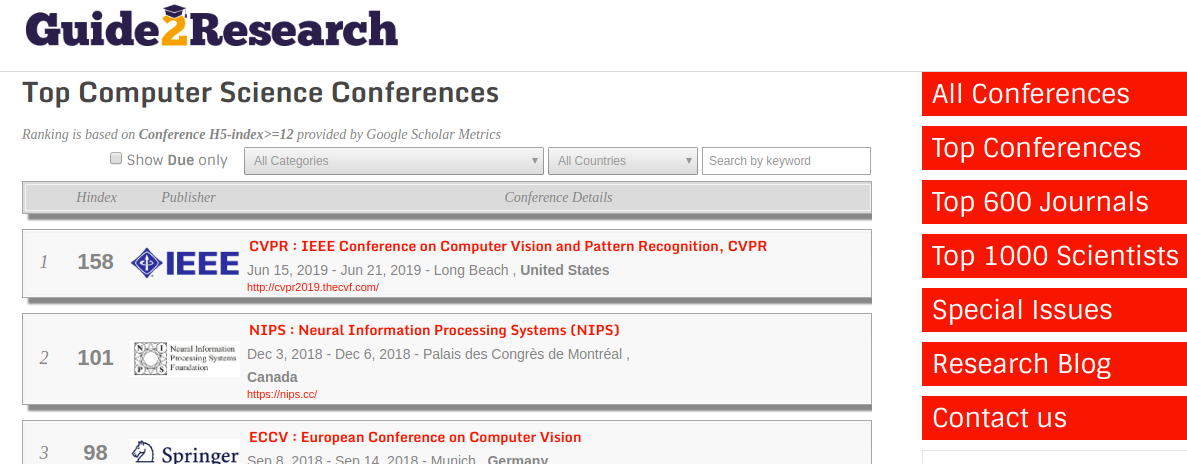
\includegraphics[scale=0.3]{images/top.png}
    \label{fig:boat1}
\end{figure}
\end{frame}

\begin{frame}{Elegir una revista}
\begin{block}{}
\begin{itemize}
    \item Reputación [-]
    \item Reputación [+]
    \item Probabilidad de rechazo [-]
    \item Probabilidad de rechazo [+]
\end{itemize}
\end{block} 
\begin{figure}[H]
    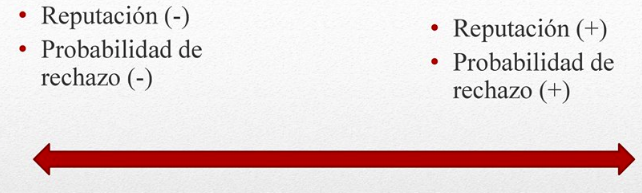
\includegraphics[scale=0.5]{images/paso1.png}
    \label{fig:boat1}
\end{figure}
\end{frame}

\begin{frame}{En la revista escogida debe: }
\begin{figure}[H]
    
\includegraphics[scale=0.5]{images/paso2.png}
    \label{fig:boat1}
\end{figure}
\end{frame}

\begin{frame}{Estructura del articulo}
\begin{block}{}
\begin{itemize}
    \item Titulo 
    \item Autores
    \item Resumen
    \item Introducción
    \item Materiales y métodos
    \item Resultados
    \item Discusión 
    \item Conclusiones
    \item Bibliografía
\end{itemize}
\end{block}   
\end{frame}


\begin{frame}{Consejos}
\begin{block}{}
\begin{itemize}
    \item Ponerse en lugar del lector.
    \item Pedir a un amigo que lo lea.
    \item Presentarlo en una conferencia.
    \item Pide ayuda a una persona con experiencia en publicar/revisa
    \item Si no sabes escribir en otro idioma, utiliza un servidor de traducción.
\end{itemize}
\end{block}   
\end{frame}


    %--------------%

   % \frame{\titlepage}

    \section{Referencias}
    \begin{frame}[allowframebreaks]
        \frametitle{Referencias}
        \printbibliography
        \begin{enumerate}
            \item [1] Introduction SCC5933 – Research Methodology in Computer Science - Instituto de Ciências Matemáticas e de Computação – USP
            \item [2] Research/Scientific Methods in Computer Science
            \item [3] Computer Science Research Methods and Writing Workshop Department of Computer Science Iowa State University \url{http://www.cs.iastate.edu/~honavar/research-methods-workshop.html}
            \item [4] Web of Science \url{https://www.fecyt.es/en/tematica/web-science}
            \item [5] Top Computer Science Conferences \url{http://www.guide2research.com/topconf/} 
            \item [6] Scimago Lab, Copyright 2007-2019. Data Source: Scopus \url{https://www.scimagojr.com/}
        \end{enumerate}
    \end{frame}
\end{document}
